
% ------------------------------------------------------------------------------

\section{Estadistica  descriptiva}

Es muy complicado sensar a toda la poblacion, entonces se procede a tomar muestras representativas. Estas muestras se toman al azar(suficiente para nosotros).

Los datos tomados se representan en el siguiente conjunto:
\[
	\{x_i\}^n_{i=1}
\]
Donde $n$ es el tamano de la muestra, siendo $N$ el de la poblacion($ < \infty$). Estos datos pueden ser cualitativos(fenero, color de ojos, etc.) o cuantitativos(numero o vectore).

\begin{definition}
	\textbf{Experimento Aleatorio}
	\begin{enumerate}
		\item Es posible repetir el experimento indefinidamente sin cambiar las condiciones.
		\item El conjunto de todos los resultados posibles se conoce como el \textbf{espacio muestral} del experimento, pero no se puede
			identificar un resultado en particular.
		\item Los resultados parecen aleatoreos a medida que se repite el experimento, pero al repetir un gran numero de veces comienza a aparecer
			un patron de regularidad. A partir del patron se puede construir un modelo matematico con el cual analizar el experimento.
	\end{enumerate}
\end{definition}

\subsection{Representacion grafica}
Primero se los representa en un grafico de forma ordenada, luego se los puede separar en pedazon mas chicos llamados \textbf{bines}, los cuales son siempre abiertos a izquierda y cerrados a derecha: $(\}$.

\begin{definition}
	\textbf{Frecuencia}
	\begin{itemize}
		\item \textbf{Frecuencia absoluta}: Numero de ocurrenciar dentro de cada bin/grupo.
		\item \textbf{Frecuencia relativa}: Representa un grupo en relacion al total, de manera que si son 3 de 200, entonces la frecuencia relativa sera $\frac{3}{200}$.
		\item \textbf{Frecuencia absoluta acumulada}: Las frecuencias absolutas sumadas de izquierda a derecha, es decir, si el grupo 1 tiene 3 y el grupo 2 tiene 5, entonces la frecuencia acumulada del grupo 2 sera 8.
	\item \textbf{Frecuencia relativa acumulada}: Igual a la frecuencia absoluta acumulada, lo que se va acumulando son las frecuencias relativas, por lo tanto el ultimo grupo tiene que tener 1. 
\end{itemize}
\end{definition}

\subsubsection{Histograma}

Util para visualizar la informacion.

\subsubsection{Poligono de frecuencias}

Usando el histograna, se trazan lineas entre cada barra.

% --- EXAMPLE IMAGES ---

\begin{figure}
	\centering
	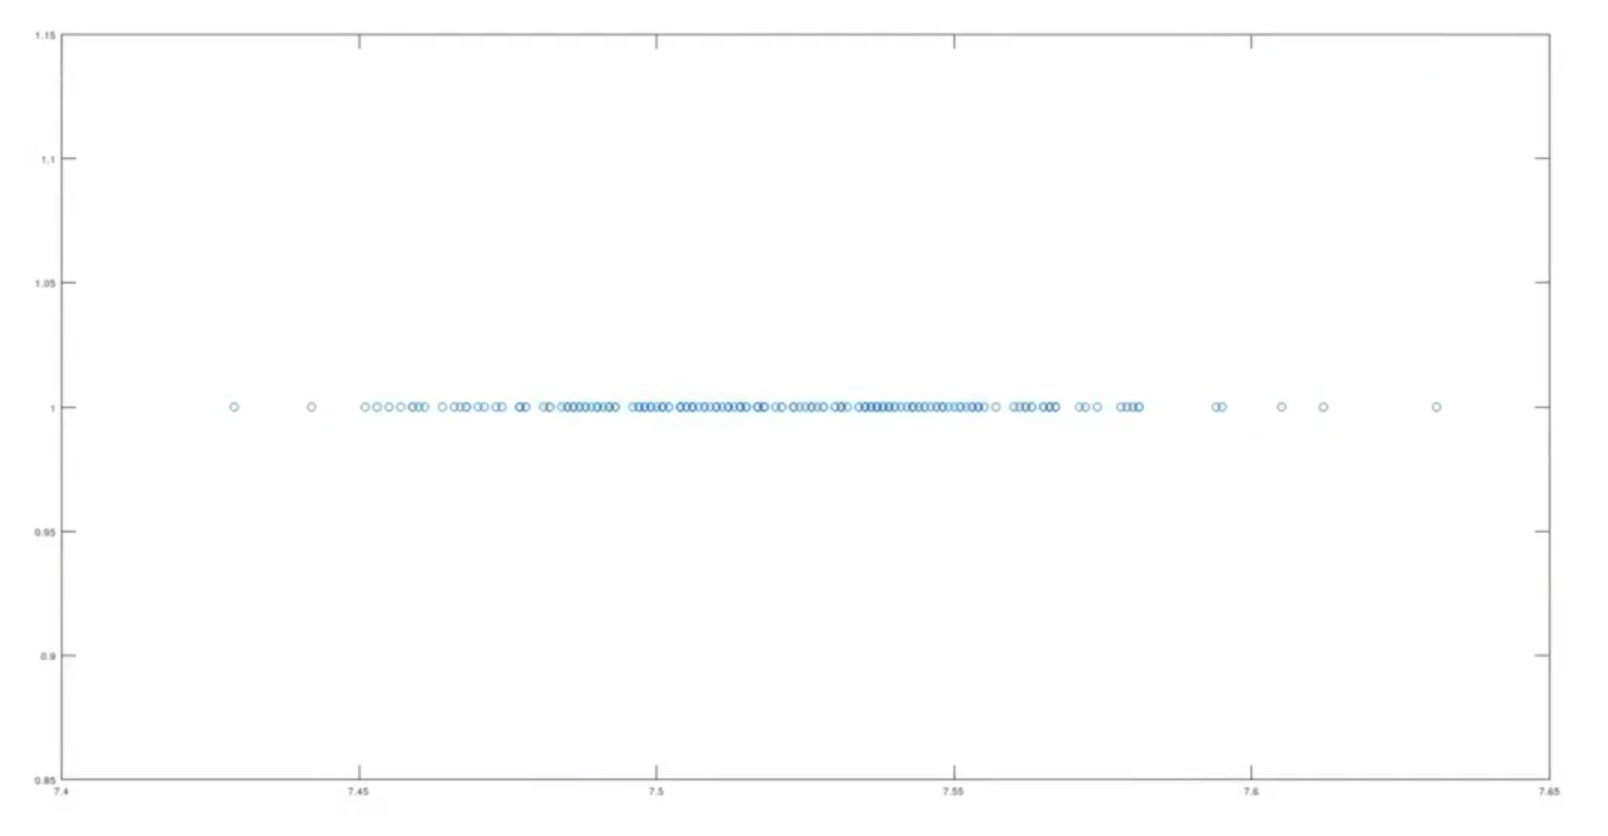
\includegraphics[width=1.0\textwidth]{graphics/dataset.png}
	\caption{Datos representados de manera ordenada}
\end{figure}
 
\begin{figure}
	\centering
	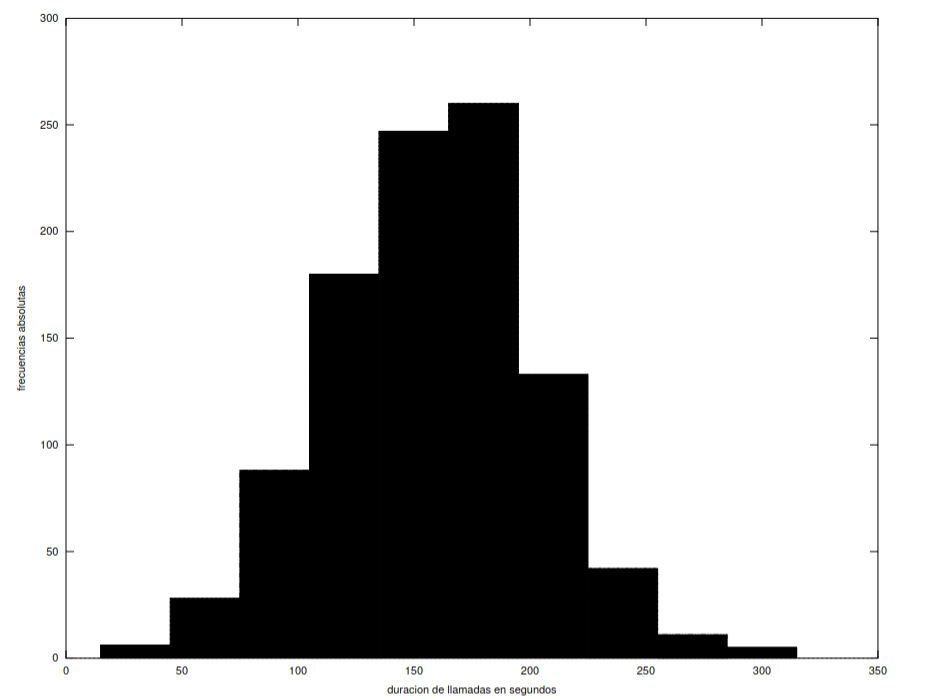
\includegraphics[width=1.0\textwidth]{graphics/histogram.png}
	\caption{Histograma de frecuencias absolutas}
\end{figure}

\begin{figure}
	\centering
	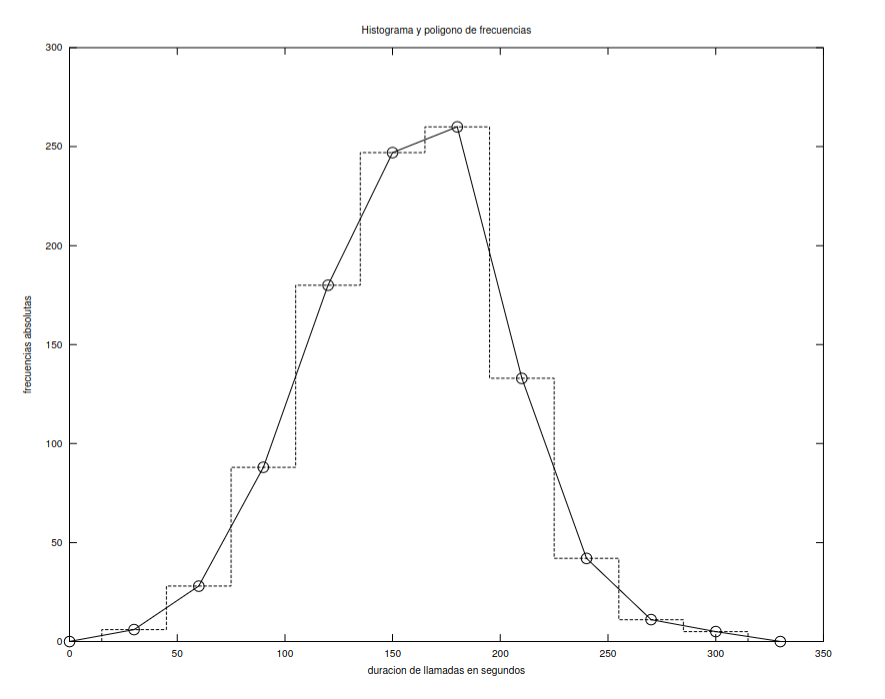
\includegraphics[width=1.0\textwidth]{graphics/poligon.png}
	\caption{Poligono de frecuencias y histograma}
\end{figure}

\subsection{Medidas de resumen}

\subsubsection{Datos sin agrupar}

\begin{definition}
	\textbf{Media arismetica}(o promedio), busca representar el "centro" de los datos de una variable cuantitativa. Sean $x_1, ..., x_n$ datos:
	\[
		\bar{x}= \frac{\sum_{i=1}^n x_i}{n}
	\]
	Notas que los datos conocidos se escriben con minuscula por convencion.

\end{definition}

\begin{definition}
	\textbf{Desvio estandard o varianza muestral}, una medida de dispersion de los datos ya que la \textbf{media arismetica} puede no ser lo que parece(diferente tamano de muestra, dispersion, etc.). Esta
	basada en la diferencia de los datos con la media
	\[
		S^2 = \frac{1}{n-1} \cdot \sum_{i=1}^n (x_i - \bar{x})^2
	\]
	Elevado al cuadrado pued puede dar negativo y no queremos eso, no se utiliza el modulo porque no es derivable. El desvio estandard es el valor de $S$.
\end{definition}

\begin{property}
$S=0 \Leftrightarrow $ Los datos son constantes(opuesto a variables).
\end{property}

\begin{definition}
	\textbf{Coeficiente de simetria}, mide el equilibrio entro los valores por debajo de la media y por arriba de la media.
	\[
		g = \frac{1}{n \cdot S^3} \cdot \sum_{i=1}^n (x_i - \bar{x})^3
	\]

	\begin{itemize}
		\item $g > 0 \rightarrow$ La variable es asimetrica derecha. 
		\item $g \approx 0 \rightarrow$ La variable es relativamente simetrica.
		\item $g < 0 \rightarrow$ La variable es asimetrica izquierda.  
	\end{itemize}

\end{definition}

\begin{definition}
	\textbf{Kurtosis}, puede diferencias las distribuciones cuando todas las anteriores coinciden. Hace referencia a que pesos tienen los datos mas alejados de la media.
	\[
		k = \frac{1}{n \cdot S^4} \cdot \sum_{i=1}^n (x_i - \bar{x})^4
	\]
El 3 es para poder interpretar la Kurtosis usando la distribucion normal como referencia.s
	\begin{itemize}
		\item $k > 0 \rightarrow$ El peso de las colas es menor al de una distribucion normal. 
		\item $k \approx 0 \rightarrow$ El peso de las colas es similar a la de una distribucino normal. 
		\item $k < 0 \rightarrow$ El peso de las colas es mayor al de una distribucion normal. 
	\end{itemize}
\end{definition}

\begin{definition}
	\textbf{Mediana}, media de tendencia central. Deja por lo menos 5\% de ;ps datos a la izquierda y el otro 50\% de los datos a la derecha(aunque no siempre se consigue). Cuando tengo un numero par de datos y no hay valor intermedio se conoce como un \textbf{caso de paridad}, hay varias maneras de obtener dicho valor(R presenta 4 opciones), pero la mas simple es sacar el promedio. 
\end{definition}

\begin{definition}
	\textbf{Cuartiles}, dividen los datos en 4, ante paridad se procede igual que la mediana(q2).
	\begin{itemize}
		\item \textbf{Primer cuartil($q_1$)}: Deja el 25\% de los datos a su izquierda.
		\item \textbf{Segundo cuartil(mediana o $q_2$)}: Deja el 50\% de los datos a su izquierda. 
		\item \textbf{Tercer cuartil($q_3$)}: Deja el 75\% de los datos a su izquierda. 
	\end{itemize}
\end{definition}

\subsubsection{Datos agrupados}
A veces los datos vienen en rangos de valores, de $L_i$(limite inferior) a $L_s$(limite superior). 
Se cuenta cuantos datos se observan en cada rango. La cantidad de datos en cada rango es la frecuencia absoluta($f_i$). 
No dan siempre lo mismo que con los datos reales, pero se aproxima.

\begin{definition}
	\textbf{Media arismetica}(o promedio), similar a datos sin agrupar:
	\[
		\bar{x}_{ag}= \frac{\sum_{i=1}^n x_i \cdot f_i}{n}
	\]
\end{definition}

\begin{definition}
	\textbf{Desvio estandard o varianza muestral}, similar a datos sin agrupar 
	\[
		S_{ag}^2 = \frac{1}{n-1} \cdot \sum_{i=1}^n (x_i - \bar{x})^2 \cdot f_i
	\]

\end{definition}

\begin{definition}
	\textbf{Mediana}, la logica es distinta, entonces se foccaliza en cuandtos datos fueron acumulados hasta cada limite superior. Se utiliza la frecuencia acumulada($F_i$). 
	Luego, elijo el intervalo que acumula el 50\% de los datos, entonces saco la mediana mediante interpolacion lineal.
\end{definition}

\begin{definition}
	\textbf{Cuartiles}, caso similar a la mediana, en caso de no tener un conjunto que acumule la cantidad exata se procede de la siguiente manera(recordar que la mediana tambien es $q_2$).
	\[
		q_{1_{ag}} = L_{i_i} + \frac{0.25 \cdot n -  F_{i-1}}{f_i} \cdot (L_{s_i} - L_{i_i})
	\]
Donde $i$ es el intervalo en el que se encuentra el cuartil. Estamos asumiendo que se distribuyen de forma equitativa(AKA interpolacion lineal).

\end{definition}

\subsubsection{Boxplot}

Combina las medidas de resumen para representar como se distribuyen los datos. 

\begin{itemize}
	\item \textbf{Alto}: La "distancia" entre $q_1$ y $q_3$ o \textbf{IQR}.
	\item \textbf{Linea horizontal}: Representa la mediana.
	\item \textbf{Lineas verticales}: Representa el minimos y el maximo de los datos.
\end{itemize}

Se puede usar para detectar errores pues es facil ver valores fuera de lugar.

\subsubsection{Outliers}

Valores considerados atipicos, usualmente indican un error en algun dato, por eso es util poder detectarlos. Se consideran atipicos debido a que se consideran lo suficientemente alejados del 50\% central. Limites de lo que se considera normal segun Tukey:

\begin{itemize}
	\item $L_w = q_1 - 1.5 \cdot (q_3 - q_1) = q_1 - 1.5 \cdot IQR$
	\item $U_w = q_3 - 1.5 \cdot (q_3 - q_1) = q_3 - 1.5 \cdot IQR$
\end{itemize}

% --- EXAMPLES IMAGES ---

\begin{figure}
	\centering
	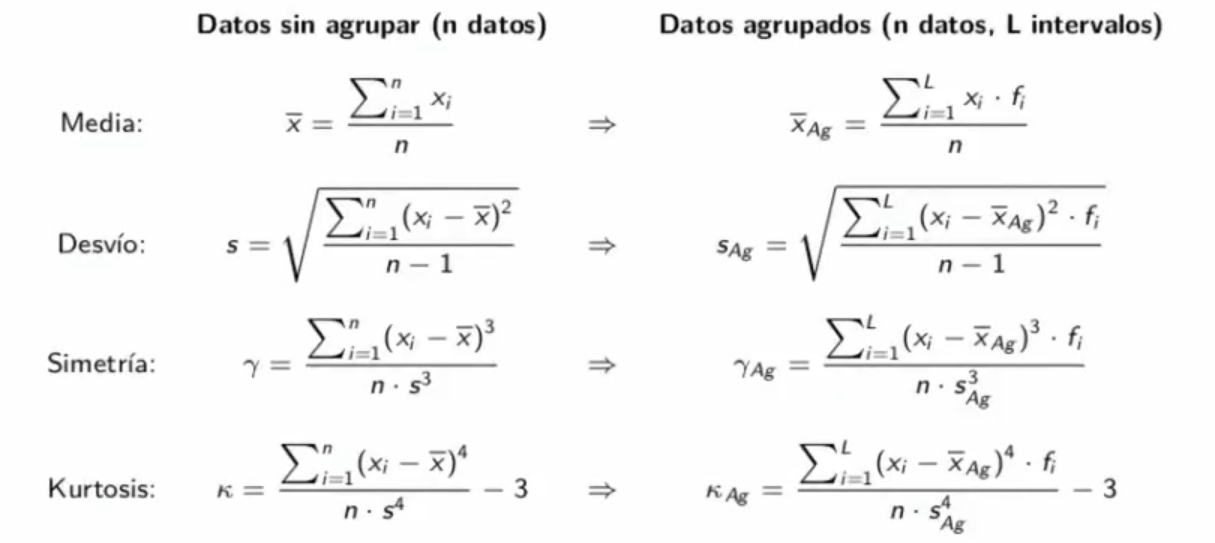
\includegraphics[width=1.0\textwidth]{graphics/desc_stat.png}
	\caption{Resumen de ecuaciones}
\end{figure}

\begin{figure}
	\centering
	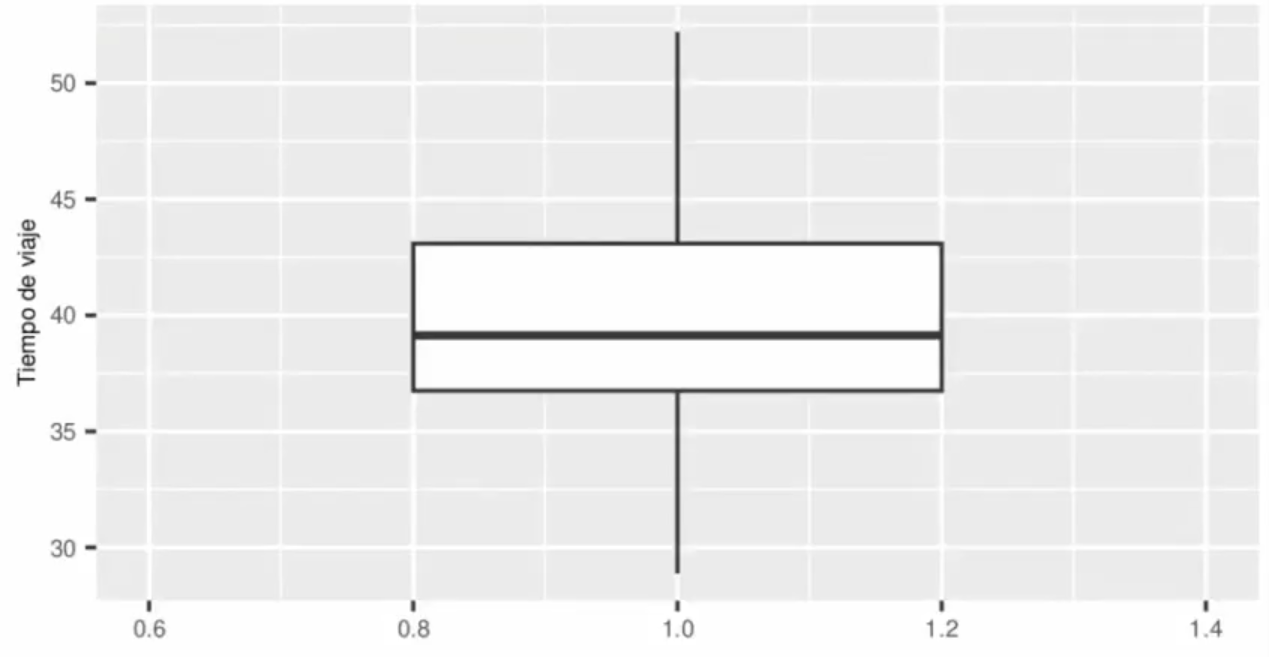
\includegraphics[width=1.0\textwidth]{graphics/boxplot.png}
	\caption{Boxplot}
\end{figure}
% ------------------------------------------------------------------------------

